\Subsection{Билет 67: Равномерная сходимость степенного ряда. Непрерывность суммы степенного ряда. Теорема Абеля.}
\begin{theorem} \thmslashn

	$R$ -- радиус сходимости, $0 < r < R$. Тогда в круге $|z| \le r$ ряд сходится равномерно.
	\begin{proof} \thmslashn
		
		$r < R \implies \sum\limits_{n = 0}^{\infty}a_nr^n$ сходится абсолютно. Для ряда $\sum\limits_{n = 0}^{\infty}a_nz^n,\ |z| \le r$ воспользуемся признаком Вейерштрасса. $|a_nz^n| \le |a_n|r^n$, $|a_n|r^n$ сходится $\implies$ по признаку Вейерштрасса $\sum\limits_{n = 0}^{\infty}a_nz^n,\ |z| \le r$ сходится равномерно. 
	\end{proof}
\end{theorem}

\begin{remark} \thmslashn

	Равномерной сходимости во всем круге может не быть.
	
	Контрпимер $R = 1$, $\sum\limits_{n = 0}^{\infty}z^n = \frac{1}{1 - z}$, хвост ряда $\sum\limits_{k = n}^{\infty}z^k = \frac{z^n}{1 - z} \not\uniconv 0$, т.к. можем одновременно приблизить числитель к единице, а знаминатель к нулю, и дробь получается сколь угодно большой.
\end{remark}

\begin{consequence} \thmslashn

	Сумма степенного ряда непрерывна в круге сходимости.
	\begin{proof} \thmslashn
		
		Возьмем произвольную точку $w$ из круга сходимости, достаточно доказать лишь непрерывность в окресности. Берем $r$, т.ч. $|w| < r < R$. Знаем, что в круге $|z| < r$ ряд равномерно сходится. Есть равномерная сходимость и каждое слагаемое это непрерывная функция$\implies$в круге $|z| < r$ сумма непрерывна$\implies$есть непрерывность суммы и в $w$. В силу произольности $w$ сумма непрерывна в любой точке $|z| < R$.
		\begin{center}
			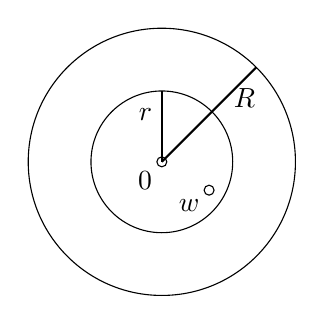
\begin{tikzpicture}[xscale=6, yscale=6]
			
			\draw[] (0, 0) circle [radius=.3pt];
			\node[below left] at (0,0) {$0$};
			
			\draw[] (0,0) circle [radius=0.2828];
			\draw[] (0,0) circle [radius=0.15];
			
			\draw [thick, -] (0,0) -- (.2,.2);
			\node[below] at (.175,.175) {$R$};
			
			\draw [thick, -] (0,0) -- (.0,.15);
			\node[left] at (.0,.1) {$r$};
			
			\draw[] (.1,-0.06) circle [radius=.3pt];
			\node[below left] at (.1,-0.06) {$w$};
			
			\end{tikzpicture}
			
		\end{center}
	\end{proof}
\end{consequence}

\begin{theorem}[Абеля] \thmslashn

	Пусть $R$ -- радиус сходимости ряда $\sum\limits_{n = 0}^{\infty}a_nz^n$ и ряд сходится при $z = R$. Тогда на отрезке $[0, R]$ ряд сходится равномерно.
	\begin{proof} \thmslashn
		
		$\sum\limits_{n = 0}^{\infty}a_nx^n = \sum\limits_{n = 0}^{\infty}a_nR^n\left(\frac{x}{R}\right)^n$. Применим признак Абеля. $\sum\limits_{n = 0}^{\infty}a_nR^n$ сходится равномерно (нет зависимости от $x$), $\left(\frac{x}{R}\right)^n \in [0, 1] \implies$равномерно огранич., $\left(\frac{x}{R}\right)^n$ монотонно убывает, тогда по признаку Абеля $\sum\limits_{n = 0}^{\infty}a_nx^n$ сходится равномерно.
	\end{proof}
\end{theorem}

\begin{consequence} \thmslashn

	$f(x) = \sum\limits_{n = 0}^{\infty}a_nx^n$, если выполнены условия теоремы, то $f(x) \in C[0, R]$, т.к. равномерная сходимость влечет непрерывность. В частности, $\lim\limits_{x \to R-} \sum\limits_{n = 0}^{\infty}a_nx^n = \sum\limits_{n = 0}^{\infty}a_nR^n$.
\end{consequence}
